
% \subsubsection{Naive Classifier}

% Four naive classification model are build according to this dataset, with $80\%$ training set and $20\%$ test set.

% \begin{table}[tbh!]
% \begin{tabular}{|l||l|l|} 
% \hline
% & Train error & Test error\\ 
% \hline
% \hline
% Logistic regression & 0.14990 & 0.15119\\
% \hline
% Random forest & 0.01998 & 0.13677\\
% \hline
% Linear discriminant analysis & 0.16213 & 0.16031\\
% \hline
% Support vector machine & 0.15488 & 0.15302\\
% \hline
% \end{tabular}
% \caption{Naive classification methods with standard settings: (1) assign positive for $p > 0.5$ in logistic regression; (2) ntree = 500 in random forest; (3) use maximum likelihood method in LDA; (4) use sigmoid kernel for SVM. }
% \label{tab:naive_model}
% \end{table}

% We compare the predictive performance of BQ with BART against the methods indicated in performance table (Table \ref{classification-performance}). Notably, the main Bayesian models that we wish to apply BQ with BART are the Gaussian process (GP) classification model with the logit link function $\sigma(p) = \log{[p/(1-p)]}$ as described in \cite{Rasmussen:2005:GPM:1162254}. Following a similar setup, given a training set $(X,y)$ and a test covariate $x_*$, we first approximate the posterior of the latent variable $f$, $p(f|X,y,x_*)$, by $q(f|X,y,x_*)$. This can be obtained either using the Laplace approximation or expectation propagation. Our predictive probability of class 1 is then 

% \begin{equation}
% p(y_* = 1|X,y,x_*) \approx \int_\mathbb{R} \sigma(f_*) q(f_*|X,y,x_*)df_*.
% \label{eq:predictprob}
% \end{equation}

% It is clear that if we had used the probit link function $\sigma(\cdot)=\Phi(\cdot)$ then (\ref{eq:predictprob}) would have a closed analytical form \cite{Rasmussen:2005:GPM:1162254}. 

% Since we do not know the exact form of the function $f$, it is not possible to compute this integral using BQ with GP, since the evaluation of the first term in (\ref{eqn:BQwithGP}) would not be attainable as we do not know the exact form of the function $f$. However, in the special where we are considering a Bayesian linear model (BLM), when $f(x) = x^Tw$, this is possible.

% Our procedure for BQ with BART is as follows. For each posterior draw $j$, we obtain $K$ functions $g_{\mbox{BART},j}^1,\ldots,g_{\mbox{BART},j}^K$ corresponding to the trees.

% \begin{table}
%     \caption{Performance of different models with respective inference methods on the classification of income bins on the "adults" dataset. The models involved are Gaussian process (GP), Bayesian linear models (BLM), support vector machines (SVM), random forest (RF) and XGBoost.}
%     \footnotesize
%     \begin{tabularx}{\columnwidth}{lcccc}
%     \hline
%     Model  & Method & Train. err.  & Test err.  \\
%     \hline
% GP (logit)      & Lapl. approx. + BART &  &  \\
%                 & Lapl. approx. + MI    &  &   \\
% GP (probit)     & Lapl. approx. &  &  \\
%                 &  Expec. prop. &  \\
% BLM             & Lapl. approx. + BART &  &  \\
%                 &  Expec. prop. + GP &  \\
% SVM             & MLE &  &     \\
% RF              & - &  &     \\
% XGBoost         & - &  &     \\
%     \hline
%     \end{tabularx}
%     \label{classification-performance}
% \end{table}

We now present a novel use of BQ-BART in the context of a different integration problem: survey sampling. We propose a new method called ``Bayesian Survey Design''. Classically, the gold standard in survey sampling is the simple random sample, i.e.~Monte Carlo. Given a set of survey respondents, estimating the population mean is equivalent to calculating the expectation of the integral of the response values (an unknown function) over the respondents who were sampled (the prior). Having phrased this problem as an integration problem, we propose the use of Bayesian Quadrature for survey design, as an alternative to the simple random sampling.

We further consider using demographic variables to model the response variable. Bayesian hierarchical models are often used in this setting to analyse survey data, in order to stabilise estimates, make them more representative, and to borrow strength when making sub-population estimates for underrepresented subgroups or locations \cite{gelman2006data}. Suppose we have a small set of survey responses consisting of interest, income, and categorical demographic variables (race, age, sex, etc). In addition, we have a much larger set of individuals for whom demographic variables are known but for whom the response variable income is unknown. We can consider surveying any of these individuals to ask them their income. Monte Carlo sampling would choose them at random, regardless of their demographics. We consider the use of Sequential Bayesian Quadrature with BART to intelligently choose the next individual to survey. We hope that this will lead to lower variance estimates with smaller sample sizes, making survey sampling more efficient. A standard refinement of simple random sampling is block (also known as stratified) random sampling. By conditioning on a variable of interest (e.g.~race), we ensure more diversity in our samples and thus obtain lower variance estimates. Our approach holds the promise of automatically ensuring a diverse sample.

\subsection{Exploratory Data Analysis}

We obtain the 2017 American Community Survey Public Use Microdata Sample (PUMS) from Wyoming \cite{ACS}, with attributes \texttt{Mobility}, \texttt{Employment}, \texttt{Sex}, \texttt{Education}, \texttt{Disability}, \texttt{Health insurance}, \texttt{Own child}, \texttt{Race}, and response \texttt{Total person income}. The goal is to predict the average income of the population. Our main interest is to estimate the average income of the working population and so we eliminate the observations with negative or zero income. Figure~\ref{fig:income} shows the histogram of distribution of income.

\begin{figure}[tbh!]
    \centering
    \vspace*{-0.1in}
    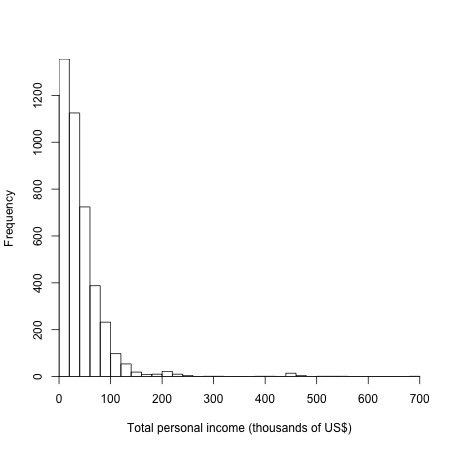
\includegraphics[width = 0.35\textwidth]{report/Writing/6.Real_Data_Sets/hist_pop.png}
    \caption{Histogram of total personal income (thousands of US\$).}
    \label{fig:income}
    \vspace*{0in}
\end{figure}

To enable experiments on a more refined model, and to test whether our approach is competitive with stratified random sampling, we categorise the population into two groups by education level: either below or higher than high school education.  

\subsection{Experimental Design}

We are first going to estimate the mean income of the whole population with some initial observations and add $M$ `best candidates' to the survey by Sequential Bayesian Quadrature with BART. Then to make the problem more complex, we stratify our data by education level and estimate the population mean for each category, using the same setup.

The details of our approach differ slightly from those explained in Algorithm \ref{alg:SQ}. Assume we are given a set of samples $\mathcal{D} = \{x_i,y_i\}_{i=1}^n$, where $x_i$ is a demographic covariate vector and $y_i$ is a real-valued label. We have a further set of candidates $\mathcal{C} = \{c_1, \ldots, c_L\}$ with known covariates but unknown responses. The goal of our design is to sequentially select $M$ individuals. Algorithm~\ref{alg:RLSQ} describes our sequential design approach. We use a discrete uniform prior and assign each candidate an equal $\frac{1}{L}$ chance to be selected. 
\begin{algorithm}[tbh!]
  \caption{Sequential Design for Survey}
  \label{alg:RLSQ}
\begin{algorithmic}
  \STATE {\bfseries Input:} \\set of labeled samples $\mathcal{D} = \{(x_i, y_i)\}_{i=1}^n$,  \\candidate set $\mathcal{C} = \{c_1, \ldots, c_L\}$ \\
  $M$ number of new samples to collect
  \FOR{$M$ iterations}
  \STATE fit BART with $\mathcal{D}$
  \STATE find posterior predictive distribution $f_{\mbox{BART}}(c)$ for all $c\in\mathcal{C}$
  \STATE find $\,c^* = \mbox{argmax}_{c} \mbox{Var}[f_{\mbox{BART}}(c)|\mathcal{D}]$
	\label{eq:maxvar}
  \STATE obtain the survey response $y_c^*$ for $c^*$
  \STATE $\mathcal{D} \leftarrow \mathcal{D}\cup \{(c^*,y^*_c)\}$
  \STATE $\mathcal{C} \leftarrow \mathcal{C}\setminus \{c^*\}$
\ENDFOR
\end{algorithmic}
\end{algorithm}

In the real world, the size of new samples $M$ could be limited by the budget or time available for conducting the survey, or other constraints.

Our BART model can be used to provide posterior predictive distributions for each of the remaining individuals whose income information is missing. Denote $f_P^k(x_i)$ as the prediction of individual $x_i$ given by the $k$th  draw from the posterior, we have the posterior estimated expected value of income 
\begin{equation}
\label{eq:mean}
    E[Y|\mathcal{D}] = \frac{1}{K}\sum_{k=1}^K\frac{1}{N}\sum_{i=1}^N f_P^k(x_i),
\end{equation}
where $N$ is the number of individuals with unknown income and $K$ is the number of posterior draws.

The posterior variance can similarly be calculated by
\begin{equation}
\label{eq:var}
    Var[Y|\mathcal{D}] = \frac{1}{K}\sum_{j=1}^K\left(\frac{1}{N}\sum_{i=1}^N f_P^j(x_i) - E[Y|\mathcal{D}]\right)^2.
\end{equation}

We compare to simple random sampling (Monte Carlo) and block random sampling, stratifying by education level. 

\subsection{Experimental Results}

Our dataset had 4,076 individuals. We begin by observing 50 random individuals, leaving the rest as a set of candidates with known demographics and unknown responses. As will be mentioned in Section~\ref{Discussion}, BART requires a minor tuning process. To achieve the best performance, we build the model with 40 posterior draws, each with 50 trees and the parameters specified in the previous section.

We compare the mean estimates from the different procedures, as well as the standard error of simple random sampling and block random sampling versus BART's posterior standard deviation calculated from Eq.~(\ref{eq:var}).

Figure~\ref{fig:poptMean} shows that by collecting further income information from 1000 individuals selected using Sequential Bayesian Quadrature, BART's estimation of average income converges much faster, with lower standard error and higher accuracy than either Monte Carlo or block random sampling. After surveying only 500 individuals, BART estimates are close to the true value, whereas simple random sampling and block random sampling remain biased even after 1000 samples.

\begin{figure}[tbh!]
    \centering
    \vspace*{-0.8in}
    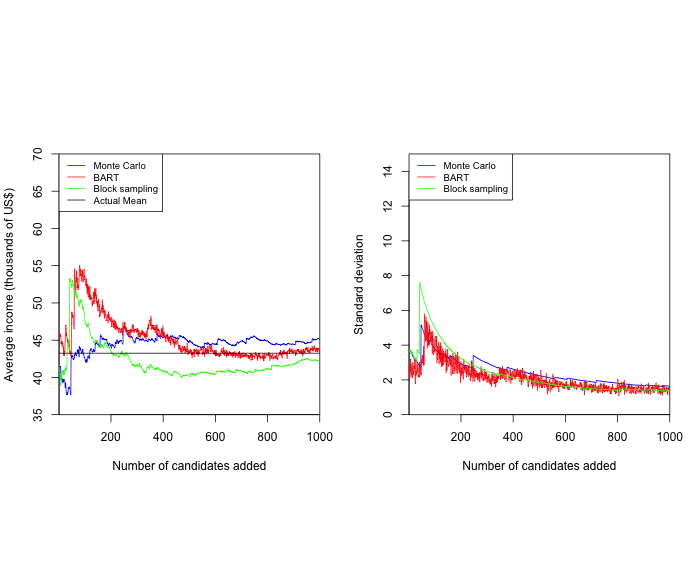
\includegraphics[width = 0.50\textwidth]{report/Writing/6.Real_Data_Sets/population.png}
    \vspace*{-0.5in}
    \caption{Estimation (left) and standard error (right) of average total income (thousands of US\$) with different sampling methods.}
    \label{fig:poptMean}
\end{figure}

To test our method in a more difficult setting, we stratify by education level, using the exact same model, but make estimates only for the average income of people with education level beyond high school. The BART-BQ design outperforms simple random sampling in Figure~\ref{fig:high+} in terms of both posterior standard deviation and estimation. Interestingly, BART-BQ still converges after only 500 samples.

\begin{figure}[tbh!]
    \centering
    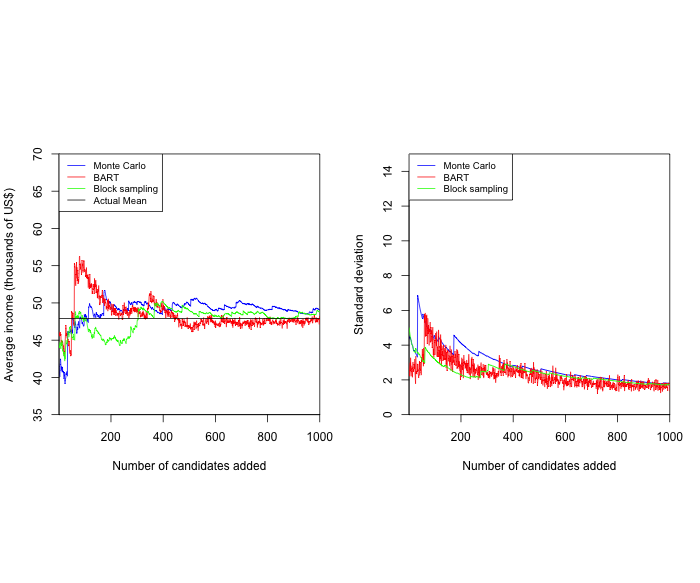
\includegraphics[width = 0.50\textwidth]{report/Writing/6.Real_Data_Sets/high+.png}
    \vspace*{-0.8in}
    \caption{Estimation (left) and standard error (right) of average total income (thousands of US\$) of population with education level beyond high school, given by different sampling methods.}
    \label{fig:high+}
\end{figure}

In the above experiments, all of the three methods provide estimates within a reasonable error margin, but BART-BQ's survey design achieves a convergence rate faster with relatively accurate estimates and lower standard error. The experiments support our proposal that when existing information and ability of obtaining further information are limited, BART-BQ with sequential design performs better than traditional random sampling methods, with little manual tuning of the method required.

Moreover, in real life, we may be able to obtain a larger initial dataset, which will lead to further improvements in BART-BQ's performance.

% \begin{table}[tbh!]
% \caption{Naive regression methods with standard settings: (1) ntree = 500 in random forest; (2) use maximum likelihood method in LDA; (3) use sigmoid kernel for SVM. (4) ntree = 50 in BART. The square root of MSE is printed.}
% \label{tab:naive_model}
% \vskip 0.15in
% \begin{center}
% \begin{small}
% \begin{sc}
% \begin{tabular}{lcccr}
% \toprule
% & Train MSE & Test MSE\\
% \midrule
% Linear regression & 0.0647 & 0.0636\\
% Random forest & 0.00911 & 0.02018\\
% LDA & 680.2146 & 658.8549\\
% SVM & 64.4301 & 63.4421\\
% %BART & 0.0239 & 0.0274\\
% \bottomrule
% \end{tabular}
% \end{sc}
% \end{small}
% \end{center}
% \vskip -0.1in
% \end{table}

% \subsection{Advanced Model Structure}

% In this section, we are going to perform \textcolor{red}{(how many?)} models with more advanced structure to obtain approximations of $E(y|x)$. 

% The comparison on MSE will be made among GP with BQ, BART with BQ, Monte Carlo method and \textcolor{red}{(other methods?)}.

% The advanced BART-BQ regression model modifies the method mentioned in BART \cite{BART}. 

% For a new data point $x$ and a BART model with functions $f^1_{j\mbox{BART}},\ldots,f^{ntree}_{j\mbox{BART}}$ in the $j$th posterior draw, each tree 

% \begin{table}[tbh!]
%     \caption{Performance of different models with respective inference regression methods on clustering coefficient on the network dataset. }
%     \footnotesize
%     \begin{tabularx}{\columnwidth}{lcccc}
%     \hline
%     Model  & Method & Train MSE & Test MSE  \\
%     \hline
% GP (logit)      & Lapl. approx. + BART &  &  \\
%                 & Lapl. approx. + MI    &  &   \\
% GP (probit)     & Lapl. approx. &  &  \\
%                 &  Expec. prop. &  \\
% BLM             & Lapl. approx. + BART &  &  \\
%                 &  Expec. prop. + GP &  \\
% SVM             & MLE &  &     \\
% RF              & - &  &     \\
% XGBoost         & - &  &     \\
%     \hline
%     \end{tabularx}
%     \label{classification-performance}
% \end{table}
